% !TeX root = ../main.tex

Dato il processo di sviluppo delle applicazioni mobile individuato nel capitolo \ref{ch:ch3} e definiti gli strumenti e task necessari, si descrive in questo capitolo come è stato automatizzato il processo adottando le moderne tecniche di integrazione continua e rilascio continuo al fine di fornire un modello di processo di sviluppo ai vari reparti aziendali che si occupano di applicazioni mobile.\\
Per la progettazione della pipeline è stato utilizzato il progetto base generato tramite il plugin Gradle KMM con lo scopo di mantenere il focus solamente sul processo e non sul prodotto. Tale progetto fornisce una applicazione essenziale sviluppata tramite KMM, comprensiva di modulo condiviso e moduli specifici sia Android che iOS.

%TODO: descrivere in breve la pipeline complessiva che si vuole sviluppare per raggiungere quali obiettivi
\begin{figure}[H]
\centering
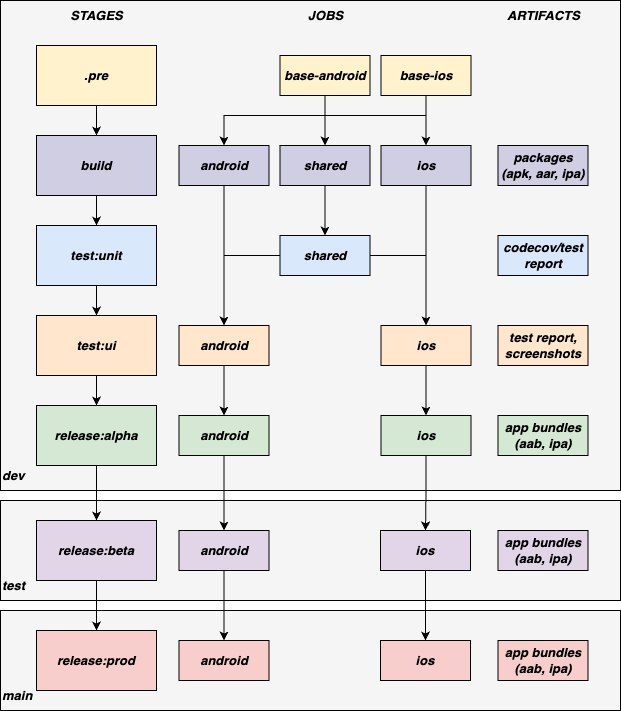
\includegraphics[width=1\textwidth]{img/tesi-11-cicd.drawio.png}
\caption{Pipeline obiettivo per la pubblicazione automatica di una applicazione Android e iOS con modulo condiviso}
\end{figure}

\section{Modello di Branching}
L'utilizzo di un adeguato flusso di lavoro è fondamentale per definire una efficiente automazione CI/CD. Con branching si intende che da uno o più flussi principali divergono altri flussi per svolgere determinati lavori per poi convergere al loro termine: in base alle modalità di apertura e chiusura di questi flussi si definiscono diversi modelli di branching.\\
Nel modello che si intende utilizzare sono presenti tre branch principali:
\begin{itemize}
    \item \textit{dev} - Flusso principale di sviluppo. Ogni modifica apportata a questo branch corrisponde al rilascio di una nuova versione \textit{alpha}. E' da questo branch che vengono aperti e chiusi nuovi branch, sia per lo sviluppo di nuove funzionalità (\textit{feature}) che per la risoluzione di bug/patch (\textit{fix}).
    \item \textit{test} - Branch modificato solamente tramite merge di modifiche provenienti dal branch \textit{dev} con lo scopo di rilasciare una nuova versione \textit{beta}.
    \item \textit{main} - Branch modificato solamente tramite merge di modifiche provenienti dal branch \textit{test} con lo scopo di rilasciare una nuova versione in produzione (\textit{prod}).
\end{itemize}

Grazie ai meccanismi di automazione a supporto della CI/CD si definiscono specifiche regole di attivazione basate sulle modifiche apportate al codice come ad esempio la modifica di un certo file su un determinato branch.

\begin{figure}[H]
\centering
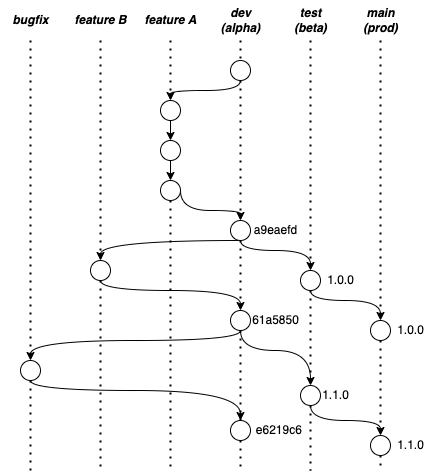
\includegraphics[width=0.6\textwidth]{img/tesi-13-branching.drawio.png}
\caption{Esempio di flusso di sviluppo adottando il modello di branching indicato}
\end{figure}

\section{Continuous Integration}

\subsection{Build}
% cache android sdk, gradle e kotlin (https://kotlinlang.org/docs/native-improving-compilation-time.html#general-recommendations)
Tipicamente la fase iniziale della integrazione continua consiste nella verifica della corretta compilazione del codice sorgente. La compilazione rappresenta un vincolo essenziale per tutte le successive fasi e per questo è definita come fase bloccante: in caso di compilazione fallita la pipeline termina senza procedere con le fasi successive.\\
Nel caso della automazione dello sviluppo di applicazioni mobile per la fase iniziale di build la pratica più diffusa è quella di validare sia la compilazione del codice, ovvero il codice condiviso (Kotlin) e il codice specifico Android (Kotlin)/iOS (Swift), che la pacchettizzazione della applicazione nei formati richiesti dalle piattaforme target (\textit{.apk}\footnote{Android Package} per Android e \textit{.ipa}\footnote{iOS App Store Package} per iOS).

\begin{listing}[H]
\inputminted{yaml}{code/4-buildjob}
\caption{Pipeline job dedicato compilazione e pacchettizzazione della applicazione Android}
\end{listing}

\begin{listing}[H]
\inputminted{ruby}{code/4-buildft}
\caption{Lane Fastlane dedicata alla fase di build tramite l'utilizzo della action Gradle}
\end{listing}

\subsection{Testing}
Dopo aver verificato la corretta compilazione e pacchettizzazione del codice segue la fase di test. Si distinguono due tipologie di testing con lo scopo di validare sia la logica applicativa (\textit{unit testing}) che l'interfaccia grafica (\textit{ui testing}).
\subsubsection{Unit Testing}

\subsubsection{UI Testing}
Analogamente agli unit test, dove si verifica l'integrità della business logic a fronte di una modifica al codice sorgente, negli UI test si verifica l'integrità dell'interfaccia grafica. I moduli per il quale deve essere testata l'interfaccia grafica corrispondono ai moduli delle applicazioni Android e iOS. I tool utilizzati per il testing dell'interfaccia grafica delle relative applicazioni sono:
\begin{itemize}
    \item \textit{Espresso}\footnote{\url{https://developer.android.com/training/testing/espresso}} (Android) -
    \item \textit{XCTest}\footnote{\url{https://developer.apple.com/documentation/xctest}} (iOS) - 
\end{itemize}
In questa specifica fase del processo tipicamente si realizzano anche degli screenshot delle applicazioni in esecuzione per essere utilizzati nelle successive fasi di pubblicazione delle applicazioni. Anche in questo caso sono necessari tool differenti per le due piattaforme, i quali sono compresi nella installazione di Fastlane:
\begin{itemize}
    \item \textit{Screengrab}\footnote{\url{https://docs.fastlane.tools/actions/screengrab/}} (Android) -
    \item \textit{Snapshot}\footnote{\url{https://docs.fastlane.tools/actions/snapshot/}} (iOS) - generato in automatico con "fastlane snapshot init" il file di supporto (SnapshotHelper.swift) e copiato il contenuto nel file autogenerato di test con xcode, poi modificato per generare gli screenshot come da documentazione fastlane
\end{itemize}

\begin{listing}[H]
\inputminted{yaml}{code/4-screenshot-ui-android}
\caption{Pipeline job dedicato al testing della interfaccia grafica e alla cattura delle schermate (Android)}
\end{listing}

\subsection{Analysis}
In questa sezione si descrivono le tecniche di analisi adottate e come queste sono state integrate nel processo di sviluppo sia per il codice sviluppato che per le dipendenze del sistema. Queste tecniche di analisi si distinguono rispettivamente in:
\begin{itemize}
    \item \textit{Static Application Security Testing} (SAST) - Analisi white-box della applicazione al fine di individuare vulnerabilità, code smell e bug.
    \item \textit{Software Composition Analysis} (SCA) - Analisi delle dipendenze di progetto con lo scopo di individuare vulnerabilità pubbliche (CVE)\footnote{Common Vulnerability and Exposure} associate ad esse.
\end{itemize}
In entrambe le tipologie di analisi è fondamentale ottenere come risultato uno o più report della scansione, in grado di descrivere in modo dettagliato eventuali "findings" trovati, ovvero l'insieme delle entità restituite dalla analisi/ricerca. I report vengono prodotti tipicamente sia in formati human-readable (es. pagina HTML) che machine-readable (es. JSON, XML, ...) per poter essere utilizzati da applicazioni terze come ad esempio servizi per centralizzare la consultazione di report eterogenei (\textit{Vulnerability Management System}).

\begin{figure}[H]
\centering
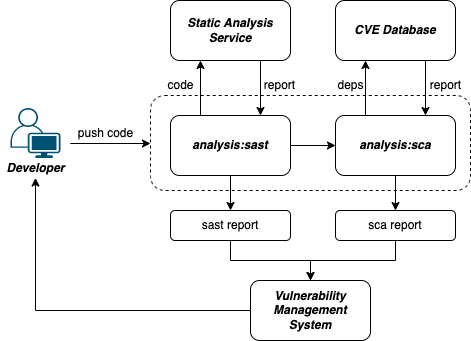
\includegraphics[width=0.7\textwidth]{img/tesi-12-sastsca.drawio.png}
\caption{Esempio tipico di integrazione della analisi statica e delle dipendenze nel processo di sviluppo automatizzato}
\end{figure}

Nel contesto aziendale Maggioli questi servizi sono messi a disposizione di tutti i team di sviluppo e mantenuti dalle figure responsabili della sicurezza informatica. Nello specifico i servizi aziendali disponibili sono:
\begin{itemize}
    \item \textit{SonarQube}\footnote{\url{https://github.com/SonarSource/sonarqube}} - Piattaforma open-source per effettuare analisi statica del codice.
    \item \textit{DefectDojo}\footnote{\url{https://github.com/DefectDojo}} - Piattaforma open-source per la gestione centralizzata delle vulnerabilità.
\end{itemize}

\subsubsection{Composizione Software}
Con composizione software si intende l'insieme di codice sviluppato da terze parti che viene incluso all'interno della applicazione, tipicamente sotto forma di import di librerie, dette dipendenze. Queste dipendenze includono a loro volta altre dipendenze e potrebbero introdurre vulnerabilità alla applicazione che le utilizza. \\
Per questo motivo è necessario analizzare le dipendenze al fine di individuare le vulnerabilità che esse introducono per essere tempestivi nel loro aggiornamento non appena vengono rilasciate delle patch di sicurezza. Il tool adottato per effettuare questa tipologia di analisi è \textit{Dependency Check}\footnote{\url{https://github.com/jeremylong/DependencyCheck}}, un tool open-source rilasciato e mantenuto da OWASP sia nella forma di plugin Gradle che come eseguibile e immagine Docker.

\begin{listing}[H]
\inputminted{yaml}{code/4-depcheckjob}
\caption{Pipeline job dedicato alla analisi delle dipendenze della applicazione Android tramite l'utilizzo del tool OWASP DependencyCheck}
\end{listing}

\subsubsection{Analisi Statica}
La fase di analisi statica viene eseguita per il codice condiviso e per il codice specifico considerando i tre moduli separatamente. I tool individuati e integrati nella fase di analisi statica del codice sono i seguenti:
\begin{itemize}
    \item \textit{Android Lint} (android, condiviso) - Tool per l'analisi statica di applicazioni Android, disponibile via CLI e via plugin Gradle (a partire dalla versione 16 ADT\footnote{Android Development Tools}).
    \item \textit{Detekt} (android, condiviso) - Tool per l' analisi statica del codice, specifico per il linguaggio di programmazione Kotlin, disponibile via CLI e via plugin Gradle.
    \item \textit{SwiftLint} (ios) - Tool per l'analisi statica del codice, specifico per il linguaggio di programmazione Swift, disponibile via CLI, e via CocoaPods.
    \item \textit{SonarQube} (android, condiviso, ios) - Client tool per l'interazione con il server SonarQube, disponibile via CLI e via plugin Gradle.
\end{itemize}

\begin{listing}[H]
\inputminted{yaml}{code/4-sastjob}
\caption{Pipeline job dedicato alla analisi statica del codice specifico Android}
\end{listing}

\begin{listing}[H]
\inputminted{ruby}{code/4-sastfastlane}
\caption{Lane Fastlane dedicata alla analisi statica del codice specifico Android}
\end{listing}

Data la funzionalità di gestione delle vulnerabilità fornita dallo stesso SonarQube e la possibilità di integrare tutte le tipologie di report prodotte sia nella fase di analisi delle dipendenze che nella fase di analisi statica del codice, si è deciso di non introdurre nel sistema l'utilizzo dei servizi forniti dalla installazione aziendale di DefectDojo.\\
Per le fasi di analisi, sia statica che dinamica, i tool hanno bisogno solo dei sorgenti e dei file di configurazione. Questo comporta il vantaggio di non dover compilare nessun file, scaricare nessun sdk, ... . Per questo motivo, dove possibile, è stata utilizzata l'immagine Docker del relativo tool come immagine per il job della pipeline.\\
Il client SonarQube utilizzato è stato dunque configurato, per poter considerare i report prodotti nelle altre fasi di analisi, agendo sui file \textit{sonar-project.properties} degli specifici moduli:
\begin{listing}[H]
\inputminted{kotlin}{code/4-sonarplugin}
\caption{Configurazione client SonarQube per il modulo condiviso (Shared)}
\end{listing}
\begin{figure}[H]
\centering
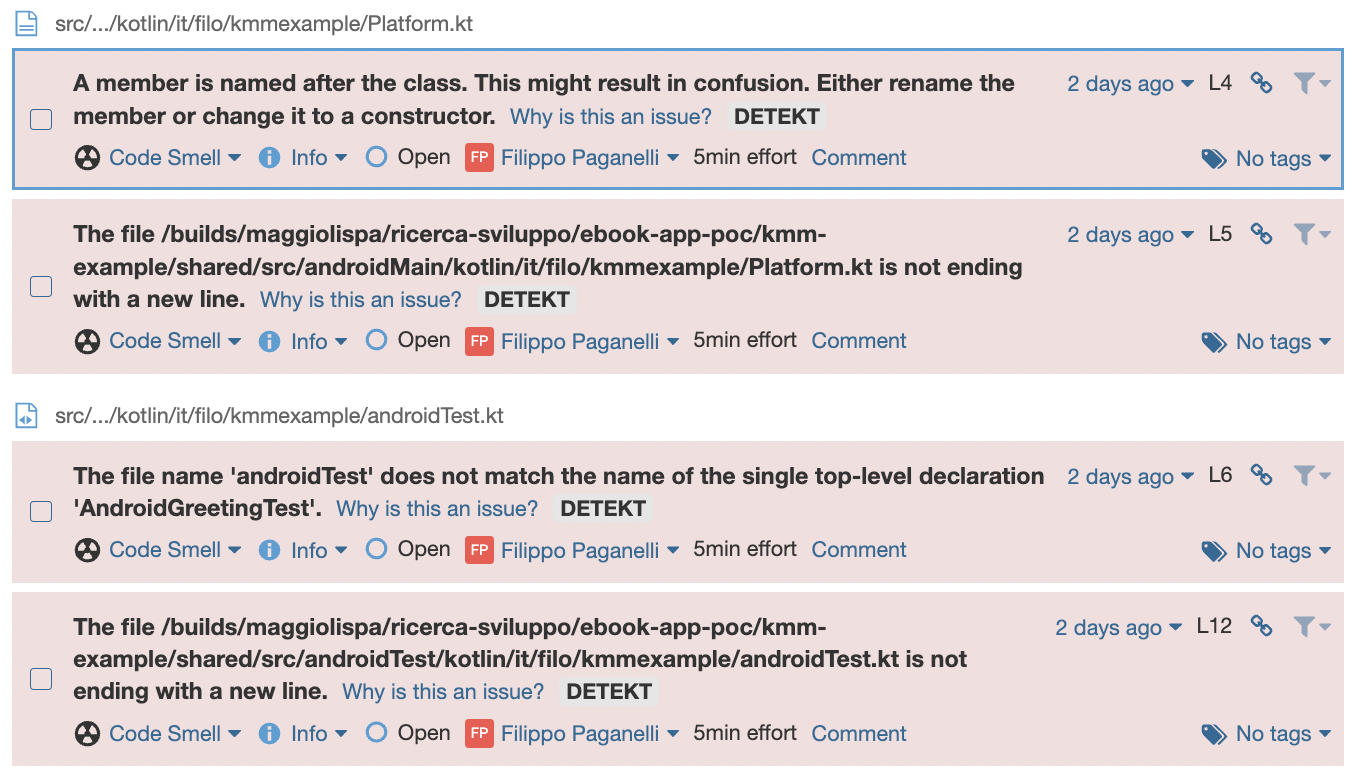
\includegraphics[width=1\textwidth]{img/Screenshot 2022-06-19 at 15.33.37.png}
\caption{Screenshot SonarQube Web UI - Esempio analisi modulo condiviso}
\end{figure}
\begin{figure}[H]
\centering
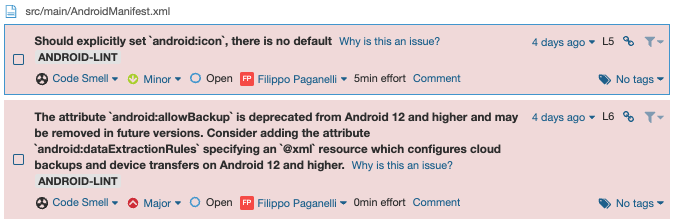
\includegraphics[width=1\textwidth]{img/Screenshot 2022-06-21 at 09.58.58.png}
\caption{Screenshot SonarQube Web UI - Esempio analisi modulo android}
\end{figure}

\subsubsection{Schedulazione Job}
Le fasi di analisi del codice possono essere introdotte nel processo di sviluppo distinguendo due modalità di esecuzione:
\begin{itemize}
    \item \textit{Sincrona} - L'analisi del codice viene eseguita ad ogni commit su uno specifico branch (in questo caso \textit{dev}). Il vantaggio consiste nella ricezione di un feedback più rapido sulla modifica apportata al codice. Lo svantaggio è dato da un incremento considerevole nel tempo di esecuzione di ogni pipeline.
    \item \textit{Asincrona} - Tramite la schedulazione delle fasi di analisi in un momento diverso da quello in cui viene apportata la modifica al codice è possibile sia ridurre i tempi di esecuzione delle pipeline che ottenere un feedback cumulativo sull'insieme delle modifiche apportate tra due esecuzioni delle pipeline di analisi del codice. Ad esempio, schedulando alla mezzanotte di ogni giorno l'esecuzione delle fasi di analisi, è possibile accedere al portale SonarQube all'inizio della giornata lavorativa successiva e pianificare gli interventi di risoluzione degli eventuali bug introdotti nella giornata precedente.
\end{itemize}

\begin{figure}[H]
\centering
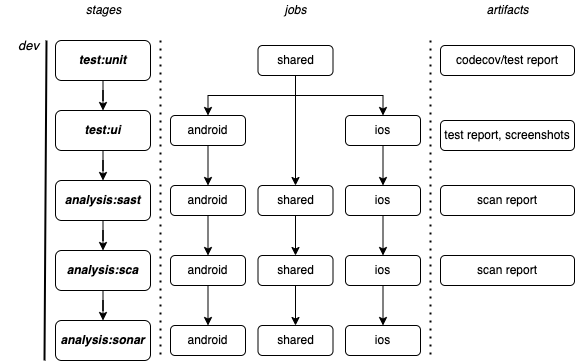
\includegraphics[width=0.88\textwidth]{img/tesi-16-cicd-scheduled.drawio.png}
\caption{Struttura della pipeline schedulata per l'analisi statica del codice}
\end{figure}

\begin{figure}[H]
\centering
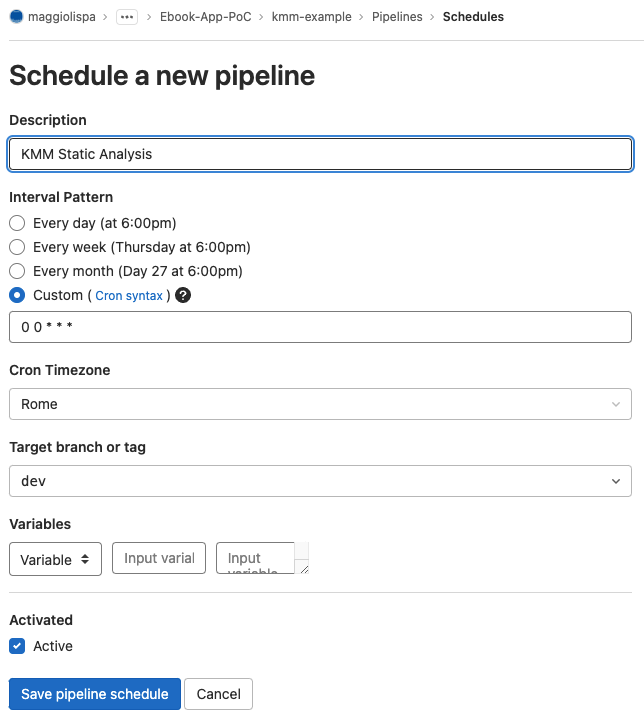
\includegraphics[width=0.8\textwidth]{img/Screenshot 2022-07-02 at 19.34.42.png}
\caption{Schedulazione pipeline GitLab: attivazione alla mezzanotte di ogni giorno sul branch \textit{dev}}
\end{figure}

\section{Continuous Delivery}

\subsection{Google Play Console}
A differenza delle applicazioni iOS, le quali richiedono due strumenti separati per la pubblicazione e per il testing, le applicazioni Android vengono gestite interamente da una unica piattaforma chiamata Google Play Console. Tramite il concetto di \textit{promozione} una specifica versione di applicazione viene infatti promossa da \textit{alpha} a \textit{beta} o da \textit{beta} a \textit{produzione}.

\begin{listing}[H]
\inputminted{ruby}{code/4-gpc-promote}
\caption{Esempio di Lane Fastlane per la promozione di un rilascio da \textit{alpha} a \textit{beta}}
\end{listing}

Per integrare correttamente nel processo di sviluppo automatizzato le fasi di pubblicazione e testing da parte degli utenti della versione Android della applicazione è necessario svolgere le seguenti azioni:
\begin{itemize}
    \item Creazione account Google Developer
    \item Creazione scheletro iniziale della app dalla piattaforma Google Play Console
    \begin{itemize}
        \item Classificazione PEGI\footnote{\url{https://pegi.info/it}}
        \item Creazione mailing-list alpha e beta tester. Tali tester per poter scaricare la applicazione tramite il link condiviso, il quale reindirizza alla pagina corretta di download sul Play Store, devono aver abilitato l'opzione "Internal App Sharing" dalle impostazioni del Play Store.
        \item Configurazione monetizzazione, pubblicità/annunci, ...
    \end{itemize}
    \item Creazione Service Account, utile a identificare/autenticare/autorizzare la applicazione creata sui servizi Google (in questa fase è necessario intervenire anche sulla piattaforma Google Cloud Platform)
    \begin{itemize}
        \item Test Connessione Fastlane-Play Store
        \begin{listing}[H]
        \inputminted{bash}{code/4-testconnessionegpc}
        \caption{Comando Fastlane per la verifica del service account creato}
        \end{listing}
        \item Setup service\_account\_key.json nei segreti GitLab per essere utilizzata dinamicamente nella pipeline senza essere versionata nei sorgenti.
    \end{itemize}
    \item Creazione chiavi, in formato \textit{Java KeyStore} (jks) per firmare l'applicazione da pubblicare
    \begin{itemize}
        \item Setup chiave jks nei segreti GitLab per essere utilizzata dinamicamente nella pipeline senza essere versionata nei sorgenti. Dato che al momento della scrittura di questa tesi GitLab non fornisce la possibilità di inserire file binari tra i segreti è stato necessario codificare in formato esadecimale la chiave generata in modo da poterla salvare come variabile testuale e decodificarla durante l'esecuzione della pipeline\footnote{\url{https://about.gitlab.com/blog/2019/01/28/android-publishing-with-gitlab-and-fastlane/}}
        \begin{listing}[H]
        \inputminted{bash}{code/4-jks}
        \caption{Creazione, codifica e decodifica della chiave JKS}
        \end{listing}
    \end{itemize}
    \item Upload manuale della prima release della applicazione. Da Agosto 2021\footnote{\url{https://developer.android.com/guide/app-bundle}} il formato di pubblicazione delle applicazioni Android \textit{aab} (Android Application Bundle) ha sostituito il formato \textit{apk}. Gli apk scaricabili e installabili sui dispositivi vengono creati automaticamente dal Play Store a partire dal aab caricato.
\end{itemize}

\subsection{TestFlight}
\begin{itemize}
    \item creazione account apple developer
    \item creare certificato per "iOS Distribution" (Certificate Signing Request \footnote{\url{https://help.apple.com/developer-account/\#/devbfa00fef7}})
    \item creazione provisioning profile. Deve essere di tipo "App Store" con il certificato appena creato, poi installazione provisioning profile (da xcode)
    \item eseguire la prima build della app in locale: dare i permessi a codesign ("always Allow" nel prompt della pwd) per accedere a "Keychain Access" in modo da poter leggere i certificati e firmare le applicazioni
    \item creazione api key per autenticarsi ai servizi "App Store connect". creo api key da "app store connect", la scarico, poi creo un file json nel formato richiesto da fastlane\footnote{\url{https://docs.fastlane.tools/app-store-connect-api/\#using-fastlane-api-key-json-file}}
    \item configurazione informazioni prima release app (come su google play console)
\end{itemize}

\subsection{Alpha Release}
% rilascio sul package registry gitlab, versionamento con l hash della commit ad ogni modifica sul branch dev. ogni versione che dal branch dev viene portata sul branch test diventa una beta release (pubblicata su testflight e google play console) e ogni versione che da test viene portata su main diventa una prod release (pubblicata su app store e google play).

\subsection{Beta Release}

\subsection{Production Release}

\section{Continuous Monitoring}
\subsection{Monitoring}
\subsection{Analytics}

\section{Infrastruttura}
% soluzione cloud ibrida: r&d su azure, i servizi condivisi sono su gcp, i servizi gitlab sono su un qualsiasi cloud provider, il runner macos è una macchina interna, ...
\begin{figure}[H]
\centering
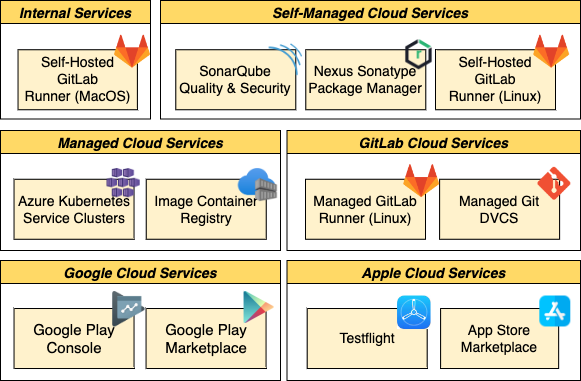
\includegraphics[width=0.8\textwidth]{img/tesi-3-infra.drawio.png}
\caption{Componenti della infrastruttura necessaria a supporto del processo di sviluppo progettato}
\end{figure}

\subsection{MacOS GitLab Runner (Self-Hosted)}
La toolchain di base per lo sviluppo di applicazioni iOS è interamente di proprietà Apple e necessita di una macchina MacOS per poter essere utilizzata definendo una serie di vincoli sia per quanto riguarda lo sviluppo locale che l'automazione del processo.
% TODO: finire l'intro di questa sezione all'utilizzo di macchina macos 
\subsubsection{Architettura Runner}
Ogni job di ogni stage definito in una pipeline viene eseguito da un componente software chiamato \textit{runner}. Tramite il modello client-server il runner interroga continuamente il server (ovvero GitLab) per ottenere le informazioni necessarie all'esecuzione dei job. La politica di scheduling dei job fra i vari runner è definita lato server ma può essere pilotata tramite il concetto di \textit{tag}.

\begin{figure}[H]
\centering
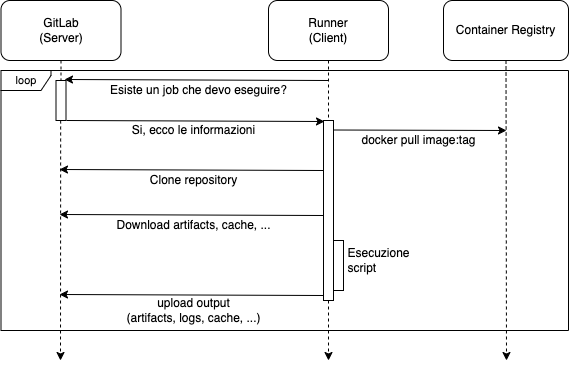
\includegraphics[width=1\textwidth]{img/tesi-17-runner.drawio.png}
\caption{Diagramma di sequenza GitLab Runner (Docker Executor)}
\end{figure}

In base a chi lo gestisce, il runner può essere:
\begin{itemize}
    \item \textit{Managed} - Runner gestito da GitLab e fornito in modalità as a service. E' soggetto ad alcune restrizioni di utilizzo che dipendono dal piano di licenza sottoscritto: tipicamente questi limiti coinvolgono il tempo di esecuzione e lo spazio di archiviazione.
    \item \textit{Self-Hosted} - Runner gestito interamente dall'utente (installazione, configurazione, registrazione, manutenzione, aggiornamento, ...). A differenza dei runner managed, questa modalità non prevede alcun vincolo di utilizzo.
\end{itemize}

Essendo il runner ad iniziare la comunicazione verso il server, uno dei principali vantaggi è quello di poterlo installare anche all'interno di una rete privata senza esporlo pubblicamente. La modalità self-hosted è stata scelta per l'installazione del runner MacOS sia per l'assenza di vincoli di utilizzo che per l'esecuzione nella rete privata aziendale Maggioli.

\subsubsection{Shell Executor}
L'esecuzione dei job avviene in modo asincrono tramite l'esecuzione di task sottoposti ad un executor. Il grado di concorrenza dell'executor, ovvero il numero di job/task che possono essere eseguiti in parallelo, è configurabile.\\
Le principali tipologie di executor sono\footnote{\url{https://docs.gitlab.com/runner/executors/}}:
\begin{itemize}
    \item \textit{Shell} - Per ogni job viene aperta una shell sulla macchina host in cui è in esecuzione il runner. Tutte le dipendenze necessarie alla esecuzione dei job devono essere installate sulla macchina.
    \item \textit{Container} - L'ambiente di esecuzione dei job è circoscritto all'interno di un container, sia nel caso dell'executor Docker che dell'executor Kubernetes. Tutte le dipendenze necessarie alla esecuzione dei job devono essere installate all'interno del container utilizzato.
    \item \textit{Virtual Machine} - I job vengono eseguiti all'interno di virtual machine, VirtualBox o Parallels, già preconfigurate.
\end{itemize}

Data la assenza di container basati su sistema operativo MacOS, l'unica opzione accettabile è quella dell'executor shell attraverso l'installazione di un runner su una macchina fisica Apple all'interno della rete privata aziendale Maggioli.

\subsubsection{Configurazione}
% installazione gitlab-runner, setup config.toml, avvio servizio
% config. ambiente: sdkman (+ java), sdkmanager, ruby, curl, fastlane, bundler, XCODE, ...

\begin{listing}[H]
\inputminted{bash}{code/4-macos-runner-setup}
\caption{Comandi bash utilizzati per l'installazione e la configurazione di un runner MacOS}
\end{listing}

\begin{listing}[H]
\inputminted{toml}{code/4-macos-runner-config}
\caption{File di configurazione (\textit{config.toml}) generato al momento della registrazione del runner}
\end{listing}

\section{Templating}
% definire la cicd in template in un progetto a parte in modo che possano essere importati nel PoC (ed essere usati da altri in futuro)
% dire come gitlab permette di farlo, quali sono i meccanismi ecc ecc
% lo stesso risultato dei gitlab template può essere ottenuto distribuendo delle github action
L'obiettivo di questo progetto di tesi non consiste solamente nella realizzazione di una pipeline di CI/CD ma consiste soprattutto nella sua progettazione in modo tale da poter essere utilizzata dai vari team in azienda che sviluppano applicazioni mobile.\\
I principali strumenti forniti dalla piattaforma GitLab a supporto del riuso delle pipeline sono:
\begin{itemize}
    \item \textit{Template} -
    \item \textit{Include} - 
    \item \textit{Extend} - Definendo lo script del job padre in modo parametrico è possibile pilotarne il comportamento tramite la definizione di variabili d'ambiente nel job figlio.
\end{itemize}